
% VLDB template version of 2020-08-03 enhances the ACM template, version 1.7.0:
% https://www.acm.org/publications/proceedings-template
% The ACM Latex guide provides further information about the ACM template

\documentclass[sigconf, nonacm]{acmart} 

%% The following content must be adapted for the final version
% paper-specific
%\newcommand\vldbdoi{XX.XX/XXX.XX}
%\newcommand\vldbpages{XXX-XXX}
% issue-specific
%\newcommand\vldbvolume{14}
%\newcommand\vldbissue{1}
%\newcommand\vldbyear{2020}
% should be fine as it is
\newcommand\vldbauthors{\authors}
\newcommand\vldbtitle{\shorttitle} 
% leave empty if no availability url should be set
\newcommand\vldbavailabilityurl{URL_TO_YOUR_ARTIFACTS}
% whether page numbers should be shown or not, use 'plain' for review versions, 'empty' for camera ready
\newcommand\vldbpagestyle{plain} 

\usepackage[utf8]{inputenc}
\usepackage{graphicx}
\usepackage{listings}
\usepackage{algpseudocode}
\usepackage{algorithm}
\usepackage{adjustbox}
\usepackage{hyperref}
\usepackage{color}
\usepackage{paralist}
\usepackage{hyperref}
\usepackage{ragged2e}
\usepackage{epsfig}
\usepackage{tikz}
\usepackage{varwidth}
%\usepackage[linesnumbered,ruled,noend]{algorithm2e}
\usepackage{fancyvrb}
\usepackage{epstopdf}
\usepackage[nomove]{cite}
\usepackage{tabularx}
\usepackage{multirow}
\usepackage{hyperref}
\usepackage{academicons}
\usepackage{xcolor}
\usepackage{dirtytalk}
\usepackage{scalerel}
\usepackage{tikz}
\usetikzlibrary{svg.path}
\usepackage{svg}
\newcommand{\orcid}[1]{\href{https://orcid.org/#1}{\includesvg[width=10pt]{orcid}}}
\definecolor{orcidlogocol}{HTML}{A6CE39}
\tikzset{
  orcidlogo/.pic={
    \fill[orcidlogocol] svg{M256,128c0,70.7-57.3,128-128,128C57.3,256,0,198.7,0,128C0,57.3,57.3,0,128,0C198.7,0,256,57.3,256,128z};
    \fill[white] svg{M86.3,186.2H70.9V79.1h15.4v48.4V186.2z}
                 svg{M108.9,79.1h41.6c39.6,0,57,28.3,57,53.6c0,27.5-21.5,53.6-56.8,53.6h-41.8V79.1z M124.3,172.4h24.5c34.9,0,42.9-26.5,42.9-39.7c0-21.5-13.7-39.7-43.7-39.7h-23.7V172.4z}
                 svg{M88.7,56.8c0,5.5-4.5,10.1-10.1,10.1c-5.6,0-10.1-4.6-10.1-10.1c0-5.6,4.5-10.1,10.1-10.1C84.2,46.7,88.7,51.3,88.7,56.8z};
  }
}

\newcommand\orcidicon[1]{\href{https://orcid.org/#1}{\mbox{\scalerel*{

\begin{tikzpicture}[yscale=-1,transform shape]
\pic{orcidlogo};
\end{tikzpicture}
}{|}}}}

\usepackage{hyperref} %<--- Load after everything else


\usepackage{biblatex} %Imports biblatex package
\addbibresource{sample.bib} %Import the bibliography file

\begin{document}
\title{Panama Papers Analysis using Graph Analytics and Embeddings}

%%
%% The "author" command and its associated commands are used to define the authors and their affiliations.
\author{Eva Chamilaki}
\affiliation{%
  \institution{Dept. of Computer Science, University of Crete \\ OramaVR}
  \city{Heraklion}
  \state{Crete}
}
\email{evacham7@gmail.com}

\author{Manos Chatzakis}
\affiliation{
    \institution{Dept. of Computer Science, University of Crete \orcidicon{0000-0002-9616-6210}\\ICS-FORTH}
    \city{Heraklion}
    \state{Crete} 
}
\email{chatzakis@ics.forth.gr}

\graphicspath{ {./figures/} }

%%
%% The abstract is a short summary of the work to be presented in the
%% article.
\begin{abstract}
The recent leak regarding Panama Papers shown that developing methods to analyze and study Fraud Detection graphs can provide significant results to improve our understanding of the data and find patterns in the available information. This report presents ways to analyze a Panama Papers dataset, using data preprocessing, graph analytics and embeddings. \\
Keywords: Fraud Detection, Panama Papers, Graph Analytics, Embeddings.
\end{abstract}

\maketitle

\section{Introduction}
This report is part of the project for the course cs484 - Complex Networks Dynamics. It presents methods to analyze a published Panama Papers dataset using data preprocessing, graph analytics and embeddings. Our contribution is summarized in the following:
\begin{itemize}
    \item We present some data preprocessing techniques, containing data cleaning and sampling in order to be able to load and analyze smaller parts of the dataset.
    \item A data analysis on the dataset based on graph analytics methods. We run a set of applicable algorithms over the graph in order to locate the most important nodes in the network.
    \item A data analysis on the dataset based on exploiting Knowledge Graph Embeddings for Fraud Detection graphs, using the most important nodes  based on the analytics. This way, we can offer methods so as to find similar nodes based on similarity search.
    \item A combination of the aforementioned approaches, utilizing the results of graph analytics for a graph embeddings database. The idea is depicted in the figure \ref{fig:work-outline}.
\end{itemize}
The rest of the report is organized as follows: Section 1 is the introduction, while Section 2 contains some basic background information. Section 3 describes how the dataset is preprocessed. Section 4 presents the work performed regarding the graph analytics. Section 5 presents the results of the embeddings creation over the Fraud Detection graph. Section 6 is the conclusion. 
\begin{figure}[htp]
    \centering
    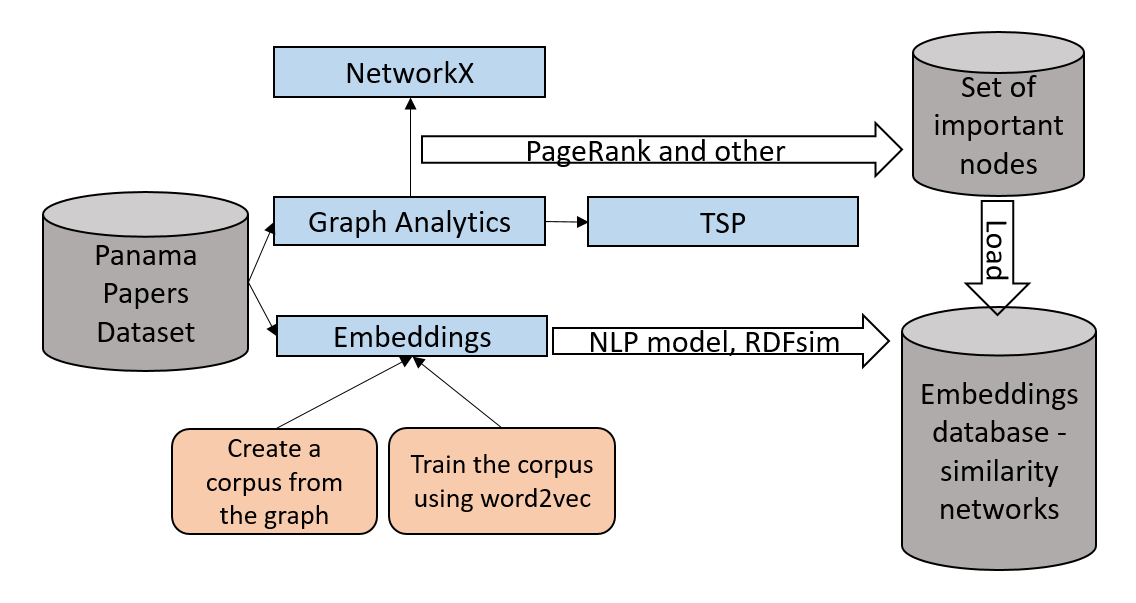
\includegraphics[width=8cm]{figures/workPlan.png}
    \caption{The work outline of this project}
    \label{fig:work-outline}
\end{figure}




%made a pass, ok
\section{Preliminaries}
In this section, basic terms are presented.\\
\textbf{[Fraud Detection Graph]} Fraud detection is a set of processes and analyses that allow us to identify and prevent unauthorized financial activity. To analyze these activities better, the data are represented as a network visualizing the relationship between the companies, people and the other type of entities.\\ 
\textbf{[Panama Papers]}
Documents with detailed financial and attorney–client information for more than 214,488 offshore entities. The documents, some dating back to the 1970s, were created by, and taken from, former Panamanian offshore law firm and corporate service provider Mossack Fonseca \cite{obermaier2017panama}.\\
\textbf{[Graph Analytics]} Graph analytics is a set of processes that are executed over a network in order to harvest information and create statistics about the graph.\\ 
\textbf{[Embeddings]} Embeddings are vector representations of words in a multidimensional vector space used to aid the problem of similarity search by exploiting cosine similarity. There is a proliferation of approaches regarding the use of embeddings over the data of Knowledge Graphs, called Knowledge Graph Embeddings. They are a part of the broad field of Natural Language Processing.

%made a pass, ok
\section{Dataset Preprocessing}
In this section we discuss general information about the dataset we used, how the preprocessing was done and what problems were encountered.
\subsection{Dataset}
The dataset we decided to use is a free access dataset containing information from offshore leaks starting back in 2013 \cite{datasetPanamaPapers}. It contains data about Panama, Pandora, Paradise papers etc. in a CSV format. For simplicity, we decided to use the data referring only to Panama papers. These data are a set of CSV files containing information about the nodes and a single CSV file that contains the edges between them. In total, there are 559600 nodes and 657488 edges.
\subsection{Graph Type} 
The form of the graph can be summarized as a set of specific types of nodes and relations between them.\\
\begin{figure}[htp]
    \centering
    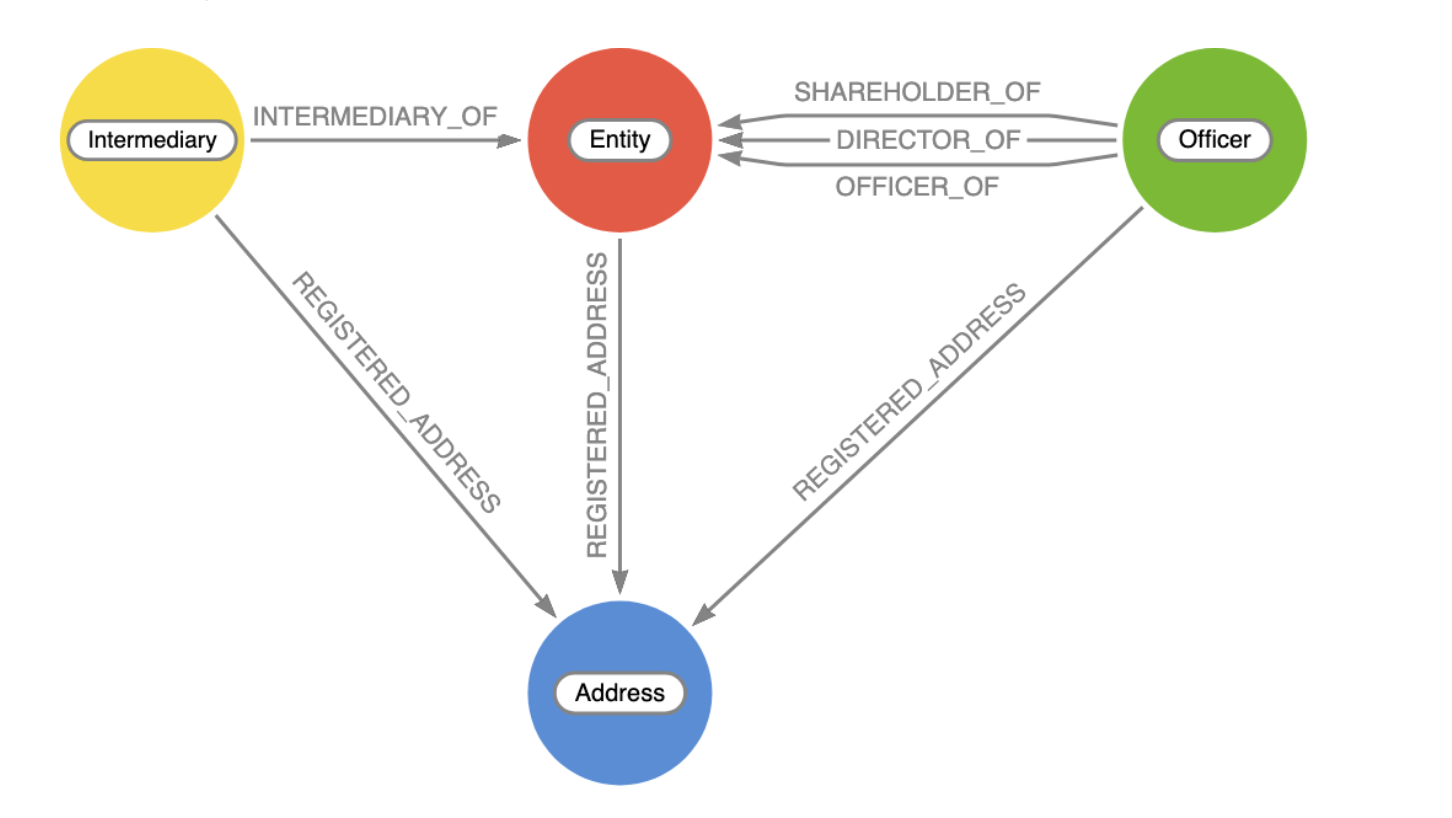
\includegraphics[width=10cm]{figures/graphType.png}
    \caption{Fraud Detection Graph}
    \label{fig:graph-type}
\end{figure}\\
Regarding the nodes, we have:
\begin{itemize}
    \item Entity: Shell company or offshore construct
    \item Officer: Proxy or real owners/shareholders/directors of a shell company
    \item Intermediary: Law firm or bank that helped create and manage the shell company
    \item Address: Registered addresses for the entities above
\end{itemize}
A summary of this schema can be seen in figure \ref{fig:graph-type}.

\subsection{Preprocessing}
The data, saved in a CSV format, contain many columns for the nodes that are not used for the graph analytics part. For the nodes, we decided to keep only the most basic information: ID, type of the node, country code and name. When the node represents an address, we decided to depict is using the name column. For the edges, we preprocessed the data to add a specific distinct link ID to every edge in the dataset, and we decided to keep: ID, SourceID, TargetID and information related to the type of the link between the nodes. We should note that any interaction and modification on the dataset was performed using CSVEditor, an open-source Java CSV editing API \cite{csvEditor}. More information about these processes are presented later on.

\subsection{Difficulties}
We should note at this point that the size of the dataset is enormous. This wasn't a problem when implementing our own methods, but for analysis purposes we had to use graph analytics tools which could not maintain nor visualize such big datasets. To tackle this problem and to also explore how we can represent subsets of an entire dataset, we developed methods to take chunks of the dataset of desired size and load them to the tools we wanted. These methods are also presented later on.
\section{Graph Analytics and Visualizations Approach}
This section presents methods used to analyse the data. These methods belong to three discrete categories: Base Dataset Analysis, Graph Analytics using Tom Sawyer Perspectives and Graph Analytics using NetworkX.

\subsection{Base Dataset Analysis}
The goal of this analysis is to find methods to get a subset of a big dataset without losing information about the form of the data. The results are used by the next analysis method for the visualization tool. The methods that will be presented have applications when we want to analyze chunks of a big data collection. They can be summarized in three approaches: The first approach just takes a sequential set of edges from the file and finds the corresponding nodes. The second follows the same logic using sampling. The third approach tries to reconstruct parts of the graph.

\subsubsection{Simple} 
This method is the most simple one. To get a subset of the dataset, we just retrieve N sequential edges from the CSV edge file, and then we go through the corresponding node data from the collection of the CSV node files. The whole process is explained in the algorithm \ref{alg:simple} in an abstract way.
\begin{algorithm}
\caption{Simple Algorithm: It takes a sequential number of edges and reconstructs a subset of the graph}\label{alg:simple}
\begin{algorithmic}

\Require $startRow \geq 0$ To be the number of the row we will start taking edges
\Require $count \geq 1$ To be the number of edges to take in total
\Require $NodeOutputFile \neq NULL$ To be the result file path of the Nodes
\Require $EdgeOutputFile \neq NULL$ To be the result file path of the Edges

\State
\State $edges \gets CSV(edgesPath)$
\State $rowID \gets 0$
\State $selectedEdges \gets edges.selectRows(startRow,startRow+count)$
\State $nodeIDs \gets hashSet()$

\State
\State{\texttt{/*Phase 1: Keep the selected edges with a rowID in a separate CSV file and save the node IDs in a set, to find them later.*/}}
\ForAll{$edges$ $e$ in  $selectedEdges$ CSV file}
    \State $currLine \gets e.getLine()$
    \State $fromID \gets currLine.getFromID()$
    \State $toID \gets currLine.getToID()$
    \State$nodeIDs.add(fromID, toID)$
    
    \State $EdgeOutputFile.writeLine$($rowID$+ , +$currLine.toString())$ \texttt{in the selected output file}
    \State $rowID \gets rowID+1$
\EndFor

\State
\State{\texttt{/*Phase 2: Traverse all CSV file that contain the nodes and save their data in a separate node CSV file.*/}}

\ForAll{CSV Files with nodes $nodeCSV$}
    \State $CSVLines \gets nodeCSV.getDesiredColumns().getLines()$
    \ForAll{$CSVLines$ $line$}
        \State $currNodeID \gets line.getNodeID()$
        
        \If{$nodeIDs.contains(currNodeID)$}
            \State $NodeOutputFile.writeLine(line.toString())$
        \Else
           \State \texttt{Ignore the current line and proceed}
        \EndIf
        
    \EndFor
\EndFor

\end{algorithmic}
\end{algorithm}
Although this method is fast and simplistic, it is obvious that the result can lead us to false conclusion about the form of the graph. This case could occur when the sample is too small.

\subsubsection{Sampling} 
In order to be more accurate on the representation of the (sub)graph, we decided to use a variation of the previous algorithm, which randomly selects N edges from the file and proceeds to find the corresponding nodes. The whole process is abstractly illustrated in algorithm \ref{alg:sampling}.
\begin{algorithm}
\caption{Sampling Algorithm: It takes a number of samples from the edges and constructs a subset of the graph}\label{alg:sampling}
\begin{algorithmic}

\Require $count \geq 1$ To be the number of samples to take from the dataset
\Require $NodeOutputFile \neq NULL$ To be the result file path of the Nodes
\Require $EdgeOutputFile \neq NULL$ To be the result file path of the Edges

\State
\State $edges \gets CSV(edgesPath)$
\State $min \gets 0$
\State $max \gets edges.getLines().size()$
\State $rowID \gets 0$
\State $randomRows \gets generateRandomNums(min,max,count)$
\State $selectedEdges \gets edges.selectRows(randomRows)$
\State $nodeIDs \gets hashSet()$

\State
\State{\texttt{/*Phase 1: Keep the selected edges with a rowID in a separate CSV file and save the node IDs in a set, to find them later.*/}}
\ForAll{$edges$ $e$ in  $selectedEdges$ CSV file}
    \State $currLine \gets e.getLine()$
    \State $fromID \gets currLine.getFromID()$
    \State $toID \gets currLine.getToID()$
    \State$nodeIDs.add(fromID, toID)$
    
    \State $EdgeOutputFile.writeLine$($rowID$ + , +$currLine.toString())$
    \texttt{in the selected output file}
    \State $rowID \gets rowID+1$
\EndFor

\State
\State{\texttt{/*Phase 2: Traverse all CSV file that contain the nodes and save their data in a separate node CSV file.*/}}

\ForAll{CSV Files with nodes $nodeCSV$}
    \State $CSVLines \gets nodeCSV.getDesiredColumns().getLines()$
    \ForAll{$CSVLines$ $line$}
        \State $currNodeID \gets line.getNodeID()$
        
        \If{$nodeIDs.contains(currNodeID)$}
            \State $NodeOutputFile.writeLine(line.toString())$
        \Else
           \State \texttt{Ignore the current line and proceed}
        \EndIf
        
    \EndFor
\EndFor

\end{algorithmic}
\end{algorithm}
This method actually gave good results, but we noticed that they did not create a large connected component of the graph (as we would expect) but instead small discrete networks of nodes. For this reason, we decided to investigate the matter even further, with a reconstruction method.

\subsubsection{Reconstruction} 
To reconstruct paths of graph we created an algorithm that randomly selects a starting node and proceeds by creating its own network in a leveled BFS manner. The method is depicted in algorithm \ref{alg:reconstruction}. 
\begin{algorithm}
\caption{Reconstruction Algorithm: Begins from a source node and recreates it's network using a leveled BFS approach. This algorithm needs to be called from several source nodes.}\label{alg:reconstruction}
\begin{algorithmic}
\Require $depth \geq 1$ The depth of the paths. Usually this is set to 3, but it can be any number above 0.
\Require $NodeOutputFile \neq NULL$ To be the result file path of the Nodes.
\Require $EdgeOutputFile \neq NULL$ To be the result file path of the Edges.
\Require $startingNodeID \geq 0$ The ID of the source node.

\State

\State $edges \gets CSV(edgesPath)$
\State $nodeIDs \gets hashSet()$

\State $levelNodes \gets list()$ of $list()$
\State $firstLevelNode \gets list()$
\State $currentLevelNodes \gets list()$

\State $firstLevelNode.add(startingNodeID)$
\State $levelNodes.add(firstLevelNode)$

\State $levelBFS \gets 0$

\State
\State{\texttt{/*Phase 1: Build the direct network of the given node using BFS-like approach.*/}}
\While{$levelBFS \leq depth$ and not $(currentLevelNodes \gets levelNodes.get(levelBFS)).isEmpty()$} 
    \State $nextLevelNodes \gets list()$
    \For{$currentNode$ in $currentLevelNodes$}
        \State $nodeIDs.add(currentNode)$
        \State $neighbours \gets CSV.groupBy(edges, currentNode).getIDs()$
        \For{$toID$ in $neighbours$}
            \If{not $nodeIDs.contains(toID)$}
                \State $nextLevelNodes.add(toID)$
            \EndIf
            \State $EdgeOutputFile.writeLine(currentNode, toID)$
        \EndFor
    \EndFor
    
    \State $levelNodes.add(nextLevelNodes)$
    \State $levelBFS \gets levelBFS+1$
\EndWhile

\State
\State{\texttt{/*Phase 2: Traverse all CSV file that contain the nodes and save their data in a separate node CSV file.*/}}

\ForAll{CSV Files with nodes $nodeCSV$}
    \State $CSVLines \gets nodeCSV.getDesiredColumns().getLines()$
    \ForAll{$CSVLines$ $line$}
        \State $currNodeID \gets line.getNodeID()$
        
        \If{$nodeIDs.contains(currNodeID)$}
            \State $NodeOutputFile.writeLine(line.toString())$
        \Else
           \State \texttt{Ignore the current line and proceed}
        \EndIf
        
    \EndFor
\EndFor

\end{algorithmic}
\end{algorithm}
Using this algorithm for large sets of nodes, we noticed the same behavior as in sampling. This means that small discrete networks of nodes is a case that occurs in the dataset many times. Although we used only one from the aforementioned approaches, the development of these algorithms helped us understand better how the data are structured. After some basic testing, we noticed that the best method to take subsets of the dataset is Sampling, thus we proceeded with this for the next step.

\subsection{Analysis and Visualization using Perspectives}

\subsubsection{Software} 
Tom Sawyer Perspectives is a graph analytics and visualization tool.

\subsubsection{Schema} 
To import the data, we needed to define a schema for our model. This schema should represent the type of the data and the interaction between them. We decided to define a simple schema. The schema contains the nodes with their attributes, and the corresponding edges, as seen in the figure \ref{fig:schema}.
\begin{figure}[htp]
    \centering
    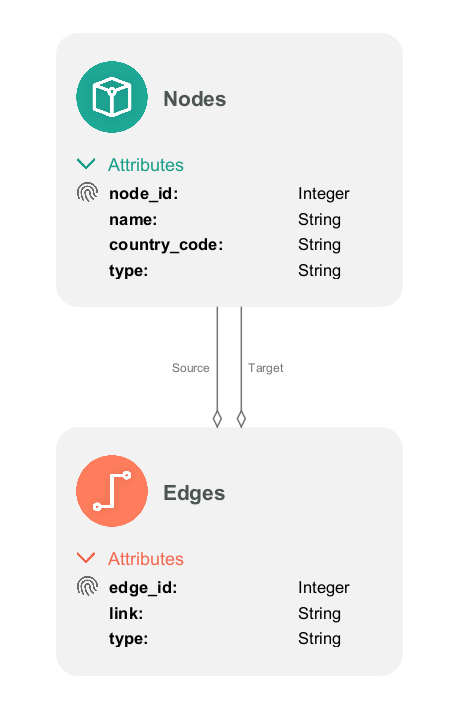
\includegraphics[width=8cm]{figures/schema.png}
    \caption{Model Schema}
    \label{fig:schema}
\end{figure}

\subsubsection{Graph}
By loading the dataset of the graph based on sampling, we managed to visualize a subgraph of the data. The subgraph consists of small (and bigger) networks of nodes. The graph is presented in figures \ref{fig:graphTSPIDs} and \ref{fig:graphTSPNames}, while the graph in full scale can be seen in figure \ref{fig:full-graph}.
\begin{figure}[htp]
    \centering
    \includegraphics[width=6cm]{figures/tspGraphID.png}
    \caption{The subgraph using the node IDs as labels, as loaded from the Perspectives previewer.}
    \label{fig:graphTSPIDs}
\end{figure}

\begin{figure}[htp]
    \centering
    \includegraphics[width=6cm]{figures/main_graph_names.png}
    \caption{The subgraph using the node names as labels, as loaded from the Perspectives previewer.}
    \label{fig:graphTSPNames}
\end{figure}

\begin{figure}[htp]
    \centering
    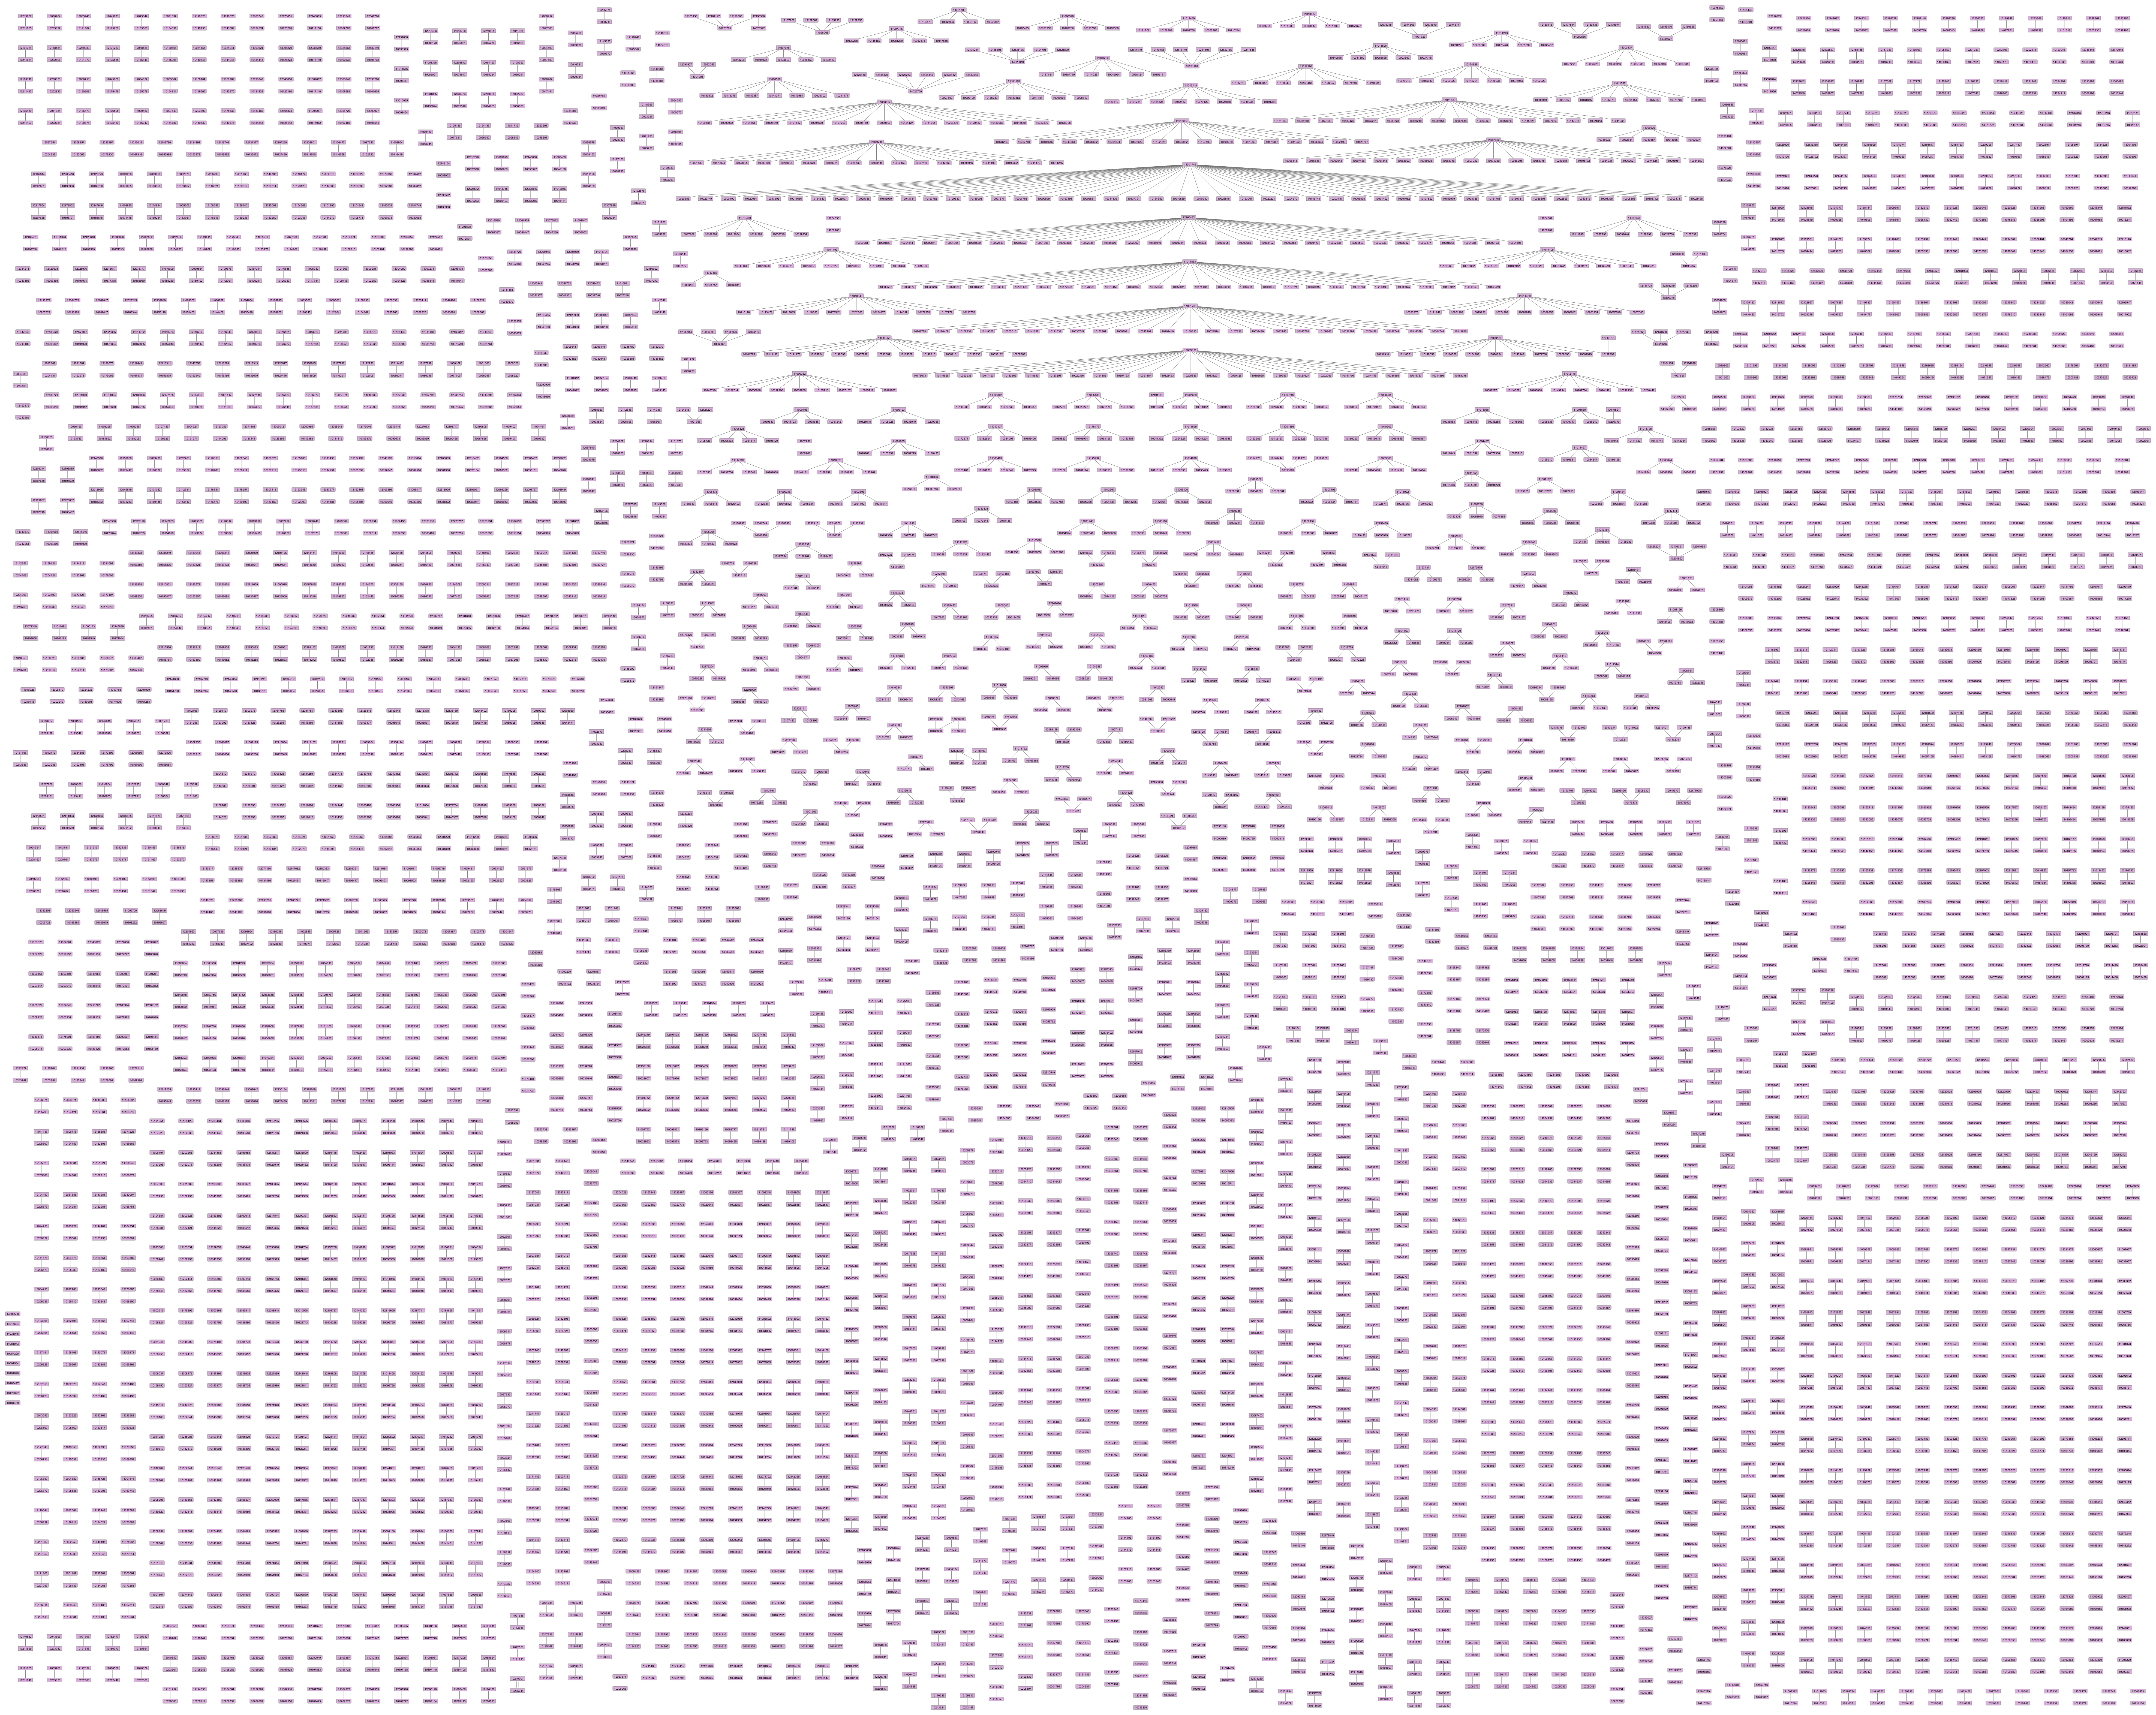
\includegraphics[width=6cm]{figures/tspGraphIDs.png}
    \caption{The complete visualisation of the subgraph, as loaded from the Perspectives previewer.}
    \label{fig:full-graph}
\end{figure}

\subsubsection{Algorithms Simulated} 
Perspectives has pre-implemented several algorithms applicable for Fraud Detection graphs. In this part of the report we present which algorithms we designed to run and provide figures about the results. As we stated before, because of the big size of the dataset, the tool could only load small subsets of it. Thus, we used the tool only for the visualizations (final results for the whole graph are presented in the next section), for a graph having around 4000 edges (using the sampling method). Profoundly, we chose to run graph algorithms that rank the nodes depending on how important they are, based in the incoming and outgoing links and the network that each node belongs. These algorithms are Eigenvector Centrality, Degree Centrality and Clustering. To run these algorithms we used the built-in analyzers of Tom Sawyer Perspectives tool as seen in figure \ref{fig:analyzersTSP}.\\
\begin{figure}[htp]
    \centering
    \includegraphics[width=6cm]{figures/analyzers.png}
    \caption{The analyzers used from the Perspectives, to apply the algorithms.}
    \label{fig:analyzersTSP}
\end{figure}
\\
\textbf{[Eigenvector Centrality]} 
Eigenvector Centrality is a measure of the influence of a node in a network. Relative scores are assigned to all nodes in the network based on the concept that connections to high-scoring nodes contribute more to the score of the node in question than equal connections to low-scoring nodes. A high eigenvector score means that a node is connected to many nodes who themselves have high scores. After running this algorithm we noticed that nodes with high score are ORION HOUSE SERVICES LIMITED, MOSSACK FONSECA CO. and OFFSHORE BUSINESS CONSULTANT (INT'L) LIMITED.
\begin{figure}[htp]
    \centering
    \includegraphics[width=6cm]{figures/tspEigenvectorGraph.png}
    \caption{A section of the eigenvector centrality graph, loaded by the Perspectives previewer.}
    \label{fig:clusterGraph}
\end{figure}\\
\textbf{[Degree Centrality]} 
Degree Centrality of a node is simply its degree—the number of edges it has. The higher the degree, the more central the node is. This can be an effective measure, since many nodes with high degrees also have high centrality by other measures and this is why both Eigenvector and Degree centrality gave the same results for the subset we loaded. Again, two \say{popular} nodes are ORION HOUSE SERVICES LIMITED and MOSSFON SUBSCRIBERS LTD.
\begin{figure}[htp]
    \centering
    \includegraphics[width=6cm]{figures/tspDegreeCentralityGraph.png}
    \caption{A section of the degree centrality graph, loaded by the Perspectives previewer.}
    \label{fig:clusterGraph}
\end{figure}\\\textbf{[Clustering]} 
Clustering is the task of grouping a set of objects in such way that objects in the same group (called a cluster) are more similar to each other than to those in other groups (clusters). After the clustering, we noticed that important nodes are ORION HOUSE SERVICES LIMITED and MOSSACK FONSECA & CO. 
\begin{figure}[htp]
    \centering
    \includegraphics[width=6cm]{figures/tspClusterGraph.png}
    \caption{A section of the clustering graph, loaded by the Perspectives previewer.}
    \label{fig:clusterGraph}
\end{figure}
A more abstract representation of the visualization created by the TSP analyzers can be seen in figure \ref{fig:tsp_analyzers}.

\begin{figure}[htp]
    \centering
    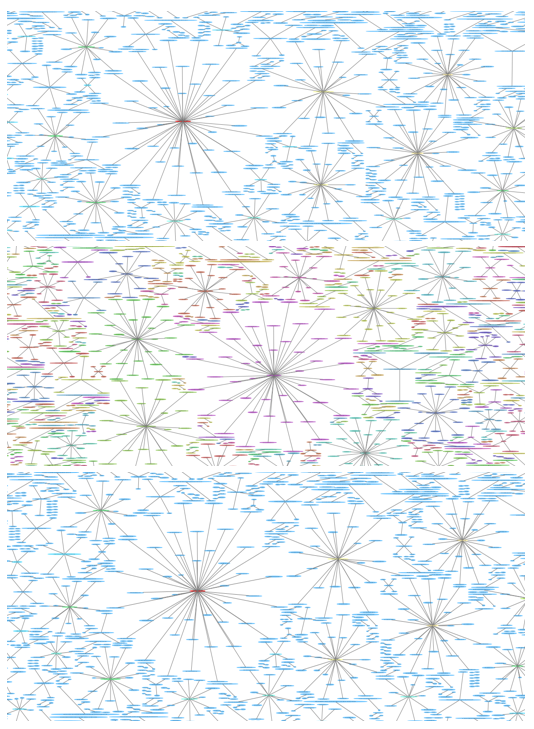
\includegraphics[width=8cm]{figures/tsp_analyzers_complete.png}
    \caption{The eigenvector, clustering and degree centrality of the subgraph, loaded by the Perspectives previewer.}
    \label{fig:tsp_analyzers}
\end{figure}

\subsection{Analysis using NetworkX}
In order to offer a complete analysis over all nodes of the network, we decided to implement some algorithms using NetworkX Python API \cite{hagberg2008exploring}.

\subsubsection{API Description}
NetworkX is an open source Python API which has implemented several graph algorithms for many kinds of graphs, while it also supports data visualization. We decided to use it as it could load the data completely.

\subsubsection{Loading the data}
As mentioned above, the data for the nodes are splitted into some csv files, while the edges are kept in a separate csv file. Thus, we implemented an initialization procedure which loads the data to NetworkX (nodes and edges) and creates a dictionary for the node IDs and their names. The process is shown in algorithm \ref{alg:networkxInit}.
\begin{algorithm}
\caption{Initialization algorithm: It loads the data from the csv and created the graph and a dictionary.}\label{alg:networkxInit}
\begin{algorithmic}

\State $IDs2Names \gets dictionary()$
\State $Graph \gets nx.directedGraph()$

\State $NodeFiles \gets [officer.csv,entity.csv,intermediary.csv,address.csv]$
\State $EdgeFile \gets edge.csv$
\State
\State \texttt{/*Add all the nodes*/}
\For{$file$ in $NodeFiles$}
    \For{$row$ in $file.rows()$}
        \State $rowID \gets row.getID()$
        \State $rowName \gets row.getName()$
        
        \State $Graph.addNode(rowID)$
        \State $IDs2Names.addMapping(rowID, rowName)$
    \EndFor
\EndFor
\State
\State \texttt{/*Add all the edges*/}
\For{$row$ in $EdgeFile.rows()$}
    \State $fromID \gets row.getFromNodeID()$
    \State $toID \gets row.getToNodeID()$
    
    \State $Graph.addEdge(fromID, toID)$
\EndFor

\end{algorithmic}
\end{algorithm}

\subsubsection{PageRank}
PageRank computes a ranking of the nodes in the graph based on the structure of the incoming and out-coming links. Although is was originally designed as a ranking algorithm for the web-pages of Google, newer versions of PageRank can aid problems from a wide domain of fields. Using PageRank to rank the nodes of our network can provide interesting results by showing the important nodes of the graphs regarding the link structure. Using NetworkX we managed to get the results for the most important nodes of the network as shown in algorithm \ref{alg:pagerank}. It needs to be stated that we decided to get only the nodes that are actual entities of the graph (i.e. we excluded the address nodes from the final results). For our computations, we simulated the process for 100 iterations and damping parameter of 0.85. Our final results are listed in the table below.
\begin{center}
\begin{tabular}{||c | c ||} %{|l|p{0.8\linewidth}|} l p{10cm}
 \hline
 Node & Pagerank \\ [0.5ex] 
 \hline\hline
 ACCELONIC LTD. (entity) & 0.00077 \\ 
 \hline
VELA GAS INVESTMENTS LTD. (entity) & 0.00060 \\
 \hline
Dale Capital Group Limited (entity) & 0.00034 \\
 \hline
BOB AGENTS LIMITED (entity) & 0.00026 \\
 \hline
GNG LTD. (entity) & 0.00023 \\
 \hline
INGELSA LTD. (entity) & 0.00020 \\
 \hline
KEINES INVESTMENTS LIMITED (entity) & 0.00019 \\
 \hline
MAGN DEVELOPMENT LIMITED (entity) & 0.00019 \\
 \hline
SITEK GROUP LIMITED (entity) & 0.00018 \\
 \hline
3 DIP S.A. (entity) & 0.00017 \\
 \hline
\end{tabular}
\end{center}
\begin{algorithm}
\caption{PageRank NetworkX: Running PageRank using NetworkX API.}\label{alg:pagerank}
\begin{algorithmic}

\State $dictionary \gets nx.pagerank()$
\State $results \gets dictionary.sort().getTopK()$
\State $printResults(results)$

\end{algorithmic}
\end{algorithm}


\subsubsection{Eigenvector Centrality}
Eigenvector Centrality is a measure of the influence of a node in a network. Relative scores are assigned to all nodes in the network based on the concept that connections to high-scoring nodes contribute more to the score of the node in question than equal connections to low-scoring nodes. The result of this algorithm is the association of a score to each node. A high score value means that a node has connections to many other nodes that also have high scores. This way we can also locate important nodes of the graph. PageRank (implemented in the previous subsection) is a variation of this method. Using NetworkX we managed to get the results using algorithm \ref{alg:evcentrality}. Our results are presented in the following table. As PageRank is a variation of this algorithm, it is normal to expect some results to be the same. Again for this approach, we decided to rule out the nodes that correspond to addresses.

\begin{center}
\begin{tabular}{||c | c||} 
 \hline
 Node & EV Centrality \\ [0.5ex] 
 \hline\hline
 ACCELONIC LTD. (entity) & 0.05063 \\ 
 \hline
VELA GAS INVESTMENTS LTD. (entity) & 0.02479 \\
 \hline
Dale Capital Group Limited (entity) & 0.02253 \\
 \hline
MAGN DEVELOPMENT LIMITED (entity) & 0.01247 \\
 \hline
DigiWin Systems Group Holding Limited (entity) & 0.01056 \\
 \hline
GNG LTD. (entity) & 0.01016 \\
 \hline
BOB AGENTS LIMITED (entity) & 0.00865 \\
 \hline
INGELSA LTD. (entity) & 0.00845 \\
 \hline
ROCKOVER RESOURCES LIMITED (entity) & 0.00840 \\
 \hline
LUK FOOK (CONTROL) LIMITED (entity) & 0.00784 \\
 \hline
\end{tabular}
\end{center}

\begin{algorithm}
\caption{EigenVector Centrality NetworkX: Running EigenVector Centrality using NetworkX API.}\label{alg:evcentrality}
\begin{algorithmic}

\State $dictionary \gets nx.pagerank()$
\State $results \gets dictionary.sort().getTopK()$
\State $printResults(results)$

\end{algorithmic}
\end{algorithm}


\subsubsection{Degree Centrality}
Another method to locate the important nodes of the graph is to calculate the fraction of nodes that the source node is connected to, either by outgoing or incoming links. Using NetworkX we managed to get results by the process depicted in algorithm \ref{alg:degree}. The results are depicted in the following table.

\begin{center}
\begin{adjustbox}{width=\columnwidth,center}
\begin{tabular}{||c | c||} 
 \hline
 Node & Degree \\ [0.5ex] 
 \hline\hline
 ORION HOUSE SERVICES (HK) LIMITED (intermediary) & 0.01254 \\ 
 \hline
MOSSACK FONSECA CO. (intermediary) & 0.00780 \\
 \hline
PRIME CORPORATE SOLUTIONS SARL (intermediary) & 0.00736 \\
 \hline
OFFSHORE BUSINESS CONSULTANT (INT'L) LIMITED (intermediary) & 0.00732 \\
 \hline
MOSSACK FONSECA CO. (SINGAPORE) PTE LTD. (intermediary) & 0.00695 \\
 \hline
MOSSFON SUBSCRIBERS LTD. (officer) & 0.00694 \\
 \hline
CONSULCO INTERNATIONAL LIMITED (intermediary) & 0.00566 \\
 \hline
MOSSACK FONSECA CO. (GENEVA) S.A. (intermediary) & 0.00534 \\
 \hline
MOSSACK FONSECA CO. (U.K.) LIMITED (intermediary) & 0.00454 \\
 \hline
MOSSACK FONSECA CO. (PERU) CORP. (intermediary) & 0.00367 \\
 \hline
\end{tabular}
\end{adjustbox}
\end{center}

\begin{algorithm}
\caption{Degree Centrality NetworkX: Running PageRank using Degree Centrality API.}\label{alg:degree}
\begin{algorithmic}

\State $dictionary \gets nx.degree()$
\State $results \gets dictionary.sort().getTopK()$
\State $printResults(results)$

\end{algorithmic}
\end{algorithm}


\subsubsection{Clustering}

\begin{algorithm}
\caption{Clustering NetworkX: Running PageRank using Clustering API.}\label{alg:cap}
\begin{algorithmic}

\State $dictionary \gets nx.clustering()$
\State $results \gets dictionary.sort().getTopK()$
\State $printResults(results)$

\end{algorithmic}
\end{algorithm}
Cluster analysis or clustering is the task of grouping a set of objects in such a way that objects in the same group (called a cluster) are more similar to each other than to those in other groups (clusters). It is a main task of exploratory data analysis, and a common technique for statistical data analysis, used in many fields, including pattern recognition, image analysis, information retrieval etc. The given result is a group of clustering coefficients, which are a measure of the degree to which nodes in a graph tend to cluster together.\\
\begin{center} 
\begin{tabular}{||c | c||} 
 \hline
 Node & Centrality \\ [0.5ex] 
 \hline\hline
Aurelio Ledergerber (officer) & 0.50000 \\ 
 \hline
FIDUCIAIRE PIRMIL SA (officer) & 0.50000 \\
 \hline
Eiger Advisory Group Inc. (entity) & 0.08333 \\
 \hline
WHELAN PROPERTIES LIMITED (entity) & 0.02381 \\
 \hline
\end{tabular}
\end{center}

\subsubsection{What do these results offer?}
The algorithms we run over our network (especially the rankings) can give us a better understanding on how the network works, which nodes are important etc. Our ranking results can show us nodes with high fraud activity over the fraud detection network, and can give us input for further investigation on the actions done by them. This idea is the base of our next section: How can we go one step further over the analysis of the graph, using different analysis methods.

\section{Embeddings Approach}
In this section we present our approach regarding the Embeddings process creation and exploitation. \\
\textbf{[General Idea]} We can use NLP (Natural Language Processing) libraries using custom corpus to produce vectors from the words than are inside the text. The pre-trained neural network of the NLP library will put the vectors of the words that are semantically close to be also close in the vector space. This way, we can aid similarity search problems. For example, we could iterate over the Fraud detection data and find the most similar off-shores based on their vectors.\\
\textbf{[word2vec]} 
To generate these vectors we exploit word2vec \cite{word2vec}, a shallow two-layer neural network model that uses a single hidden layer for producing word embeddings. The input is a text (in our case triples of fraud detection data) while  the output is a multidimensional vector (usually with over a hundred of dimensions) for each unique word (in our case nodes) that appears in the text. The vectors it produces are based on the co-occurrence of words (in our case node names and link types) in context windows of a given size, and it aims at grouping the vectors of similar words (based on their co-occurrence) closely in the vector space. 
The recommended value of the size of context window depends on the word2vec model, e.g., in the skip-gram model, that value is usually around 10. However, in our case we use a context window of size 3, since for an entity we produce one sentence for each of its triples (i.e., each sentence contains 3 words), which means that we capture similarities based on the co-occurrence of nodes and the links between them.

\subsection{Graph Embeddings}
The basic challenge when using embeddings for graphs is to transform the graph into a text corpus, in order to load it to the corresponding library. The most used method is to represent the graph as a set of triples, where each triple is in the form of NODENAME LINKTYPE NODENAME. Such files can be produced easily and be used as a corpus. In the following sections, we describe how we transformed the Fraud Detection graph into corpus and how we trained the model.

\subsection{Vocabulary Creation}
For the vocabulary, we developed an algorithm that transforms the graph into sentences of triples representing the connections between the nodes. The challenge was to gather all the node files and replace the nodeIDs with their actual names. A summarization of the process is shown in algorithm \ref{alg:vocab}.
\begin{algorithm}
\caption{Vocabulary Creation Algorithm: It produces a text corpus from the edges of the graph}\label{alg:vocab}
\begin{algorithmic}
\Require $corpusPath \neq NULL$ To be the output file for the corpus

\State
\State{\texttt{/*Phase 1: Create a mapping for the nodeIDs with their names*/}}
\State $IDs2names \gets HashMap<Int,String>()$

\For{$currCSV$ in $CSVfiles$}
    \State $lines \gets currCSV.getDesiredColumns().getLines()$
    \For{$line$ in $lines$}
        \State $lineID \gets line.getID()$
        \State $lineName \gets line.getName()$
        \State $IDs2Names.put(lineID, lineName)$
    \EndFor
\EndFor

\State
\State{\texttt{/*Phase 2: Create the corpus using the edges and the map*/}}

\State $edges \gets CSV(edgesPath)$
\State $lines \gets edges.getLines()$

\For{$line$ in $lines$}
    \State $fromID \gets line.getFromID()$
    \State $toID \gets line.getToID()$
    \State $link \gets line.getLink()$
    
    \State $fromIDName \gets IDs2Names.get(fromID)$
    \State $toIDName \gets IDs2Names.get(toID)$
    
    \State $corpusPath.writeLine(fromIDName + link + toIDName)$
\EndFor

\end{algorithmic}
\end{algorithm}

\subsection{Embeddings Training}
\subsubsection{Skip-gram model} 
For computing the embeddings,  we use the skip-gram model of word2vec. We decided to use this model instead of the Continuous-Bag-of-Word (CBOW) model of word2vec, since in most cases Skip-gram outperforms CBOW for large datasets. Skip-gram model uses unsupervised learning techniques for finding the most related words (in our case Fraud Detection entities) for a given word, that is, it uses a target word for predicting the context words. 
In particular, given a sequence of training words, say $word_1$, $word_2$ , ... , $word_T$, and a context window of size $c$, the skip-gram model tries to maximize the average log probability, which follows:

\begin{equation}
\frac{1}{T} \sum_{t=1}^{T} \sum_{-c\leq j \leq c, j\neq 0}^{} \log{p(word_{t+j}|word_t)}.
\end{equation}

The probability $p(word_{t+j}|word_t)$ is computed using the softmax function:

\begin{equation}
p(word_{t+c}|word_t)=\frac{exp(v^{\prime T}_{word_{t+c}} v_{word_t})}{\sum_{m=1}^{|U|} exp(v^{\prime T}_{words_{m}} v_{words_t})}.
\end{equation}

In the above formula, $v^{\prime}$ and $v$
are the input and the output vectors of a word $word$, whereas $|U|$ is the number of unique words in our vocabulary (text corpus). \\
\subsubsection{Implementation} 
Our implementation exploits the SkipGram model of word2vec to create the embeddings, as shown in the algorithm \ref{alg:train}.
\begin{algorithm}
\caption{Embeddings Training Algorithm}\label{alg:train}
\begin{algorithmic}

\Require $corpusPath \neq NULL$ To be the input file for the corpus
\Require $datasetPath \neq NULL$ To be the output file for the embeddings

\State $vectors \gets model.trainWithDefaults(corpusPath)$

\State $vectors.removeLinks()$
\State $vectors.removeAddresses()$

\State $RDFsim.createDataset(vectors)$

\end{algorithmic}
\end{algorithm}

\subsection{Similarity Search over Fraud Detection Data}
\subsubsection{Similarity Search}  
One of the most important data mining tasks is similarity search i.e. “Given an embedding of a word in a multidimensional space, give me the most similar words of it using the vector space, Euclidean distance and cosine similarity”. The aforementioned term is contextualized for embeddings similarity search.\\
\subsubsection{Similarity Method for computing the K most similar nodes}
For finding the K most similar entities to a given entity, we employ the cosine similarity score of their vectors.  
The cosine similarity between  two vectors $v^{\prime}_{vec_1}$ and $v^{\prime}(vec_2)$ (each vector corresponds to a single word) is defined as: 

\begin{equation}
    \cos(\theta)_{vec_1,vec_2}={ {v^{\prime}_{vec_{1}}} \cdot  {v^{\prime}_{vec_{2}}}  \over \| {v^{\prime}_{vec_{1}}} \|\| {v^{\prime}_{vec_{2}}} \|}.
\end{equation}

The score ranges from -1 (i.e.,  two vectors are exactly opposite) to 1 (i.e., two vectors are exactly the same). 
To compute the K most similar entities to a given word $word$, we rank the rest words according to their  $\cos(\theta)_{vec,vec^{\prime}}$ score in descending order, 
and we keep the words placed in the first $K$ positions in the ranking (i.e., the $K$ most similar words to $word$). 

\subsection{RDFsim Engine Exploitation}
\subsubsection{RDFsim} 
RDFsim \cite{rdfsim} is a similarity search engine over semantic Knowledge Graph data (mainly from DBpedia) developed and published by Manos Chatzakis, Michalis Mountantonakis and Yannis Tzitzikas in Summer 2021. Although it is designed and tuned for semantic data, we managed to port custom data using some of the RDFsim+ feautures. These features can load any corpus (even non-semantic data) and their embeddings, and manage to create similarity networks. RDFsim exploits the embeddings by implementing a BFS-like algorithm in order to build and visualize similarity graphs using a JavaScript framework. RDFsim is an open-source, under development tool \cite{RDFsimcurrent, RDFsimdemo}. The tool manages to create the networks with it's own BSF-like method, shown in algorithm \ref{alg:graph}. An outline of the embedding creation and RDFsim exploitation is presented in figure \ref{fig:embedding-creation}.

\begin{figure}[htp]
    \centering
    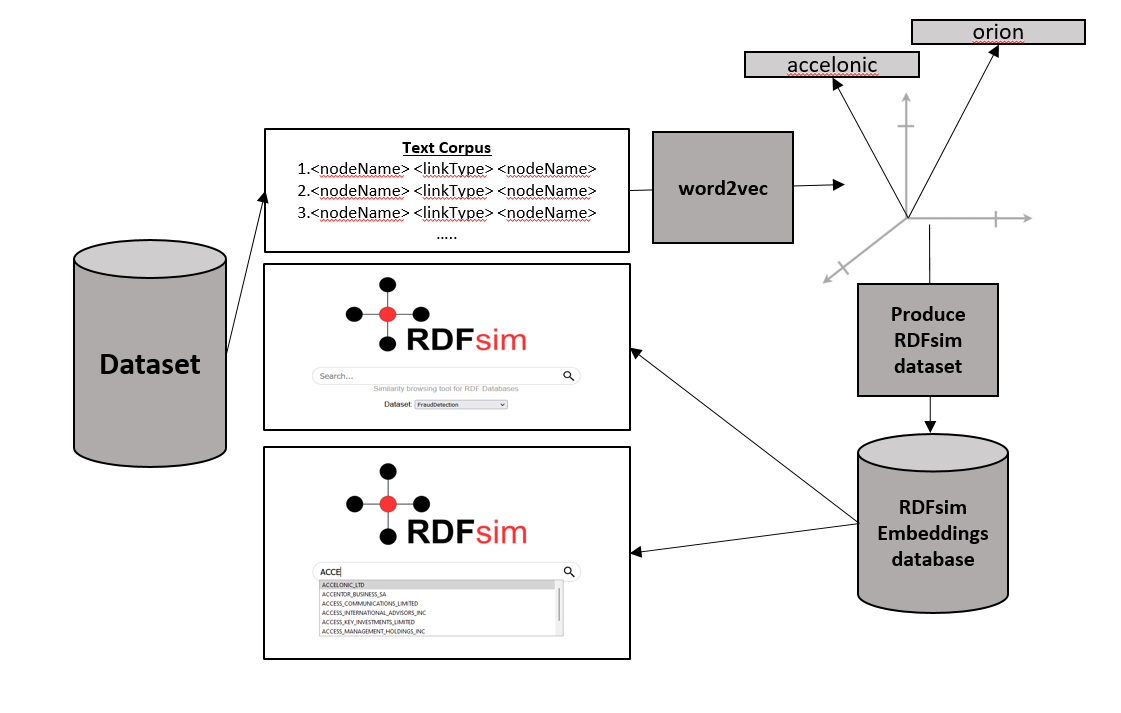
\includegraphics[width=8cm]{figures/embeddingsProcess.png}
    \caption{The process of producing the graph embeddings and the RDFsim exploitation}
    \label{fig:embedding-creation}
\end{figure}

\begin{algorithm}
\caption{Creating the similarity graph $G$ for the selected entity $e_{sel}$.}
\label{alg:graph}
\begin{algorithmic}

\Require Entity $e_{sel}$, depth $L$, number of similars $K$, Entity Index $ei$

\State \texttt{The similarity graph starting $G$  from entity $e$ by using specific $L$ and $K$}

\State \texttt{Initialize Graph}
\State $Graph~G \{$ \\$~~~~V \leftarrow \emptyset$, \\$~~~~E\leftarrow \emptyset$ \\
$\}$ 
\State $level \leftarrow 1$ 
\State $V(level) \leftarrow \emptyset$
\State \texttt{Add the selected entity as the first node}
\State $G.V \leftarrow G.V \cup \{e_{sel}\}$ 
\State $V(level) \leftarrow V(level) \cup \{e_{sel}\}$ 
\State \texttt{Follow a BFS-like approach}
\While{$level\leq L$ and $V(level) \neq \emptyset$}
    $V(level+1) \leftarrow \emptyset$
	\State \texttt{Traverse each node $e$ of the current $level$}
	\ForAll{$e \in V(level)$}
	\State $similars(e,K) \leftarrow ei.getSimilarEntities(e,K)$
	\State \texttt{Traverse  the top-K to similar entities of $v$ and create the corresponding nodes/edges (if they do not exist)}
	    \ForAll{$e^{\prime} \in similars(e,K)$}
	        \If{$e^{\prime} \notin G.V$}
	            \State $G.V \leftarrow V \cup  \{e^{\prime}\}$ 
	            \State $G.E \leftarrow G.E \cup \{e,e^{\prime}\}$ 
	            \State $V(level+1) \leftarrow V(level+1) \cup { \{e^{\prime}\}}$
	              
            \ElseIf{$\{e,e^{\prime}\} \notin G.E$}
	            \State $G.E \leftarrow G.E \cup \{e,e^{\prime}\}$
            \EndIf
	    \EndFor
    \EndFor
\EndWhile
	    
\State $level \leftarrow level+1$
	   
\State \texttt{return $G$} 
	
\end{algorithmic}
\end{algorithm}

\subsubsection{How can RDFsim be used for our data} 
After producing the embeddings and the RDFsim-supported dataset, we can load our data directly into the search engine. Then, we can start doing queries on the data. Our main idea was to provide another method for finding relationships between companies and people that are inside the dataset. Using RDFsim, we can create large similarity networks of companies and people, and if the parameter tuning is good enough, we can find relations between companies and people that are not easily discoverable through classic graph analytics method. For example, if two companies have relationships with people that have some kind of relationships (through other nodes), word2vec understands that and the vectors of the companies will be closer into the vector space. Also, using word2vec and RDFsim algorithms, we managed to load the whole dataset and produce embeddings for all the companies that have a significant number of relationships. We decided to do that because it has really efficient results, and because we decided that it is better to give results for the most important nodes of the dataset (i.e. nodes with many connections). Another good point for using RDFsim is that the parameters of the training can be easily tuned, while the model is scalable for better and more powerful systems. Some use cases about the idea of implementing knowledge graph embeddings algorithms to fraud detection graphs are presented in the next section. 

\subsubsection{Examples and Use Cases} 
Our port of the data and the local build of RDFsim is easily accessible though it's official development GitHub repository. In this section, we present some basic examples on how we can interact with the Fraud Detection data. For the use cases, we decided to examine the similarity networks of the nodes that had high scores in the algorithms implemented from NetworkX.
Thus, we will explore the similarity graphs of the following nodes:
\begin{itemize}
    \item ACCELONIC LTD. (entity node)
    \item VELA GAS INVESTMENTS LTD. (entity node)
    \item ORION HOUSE SERVICES (HK) LIMITED (intermediary node)
    \item (at this point, we can search and create the similarity network of any node we want)
\end{itemize}
\textbf{[ACCELONIC LTD.]} For this entity, the direct network leads us to the corresponding star-graph, consisting of nodes that are probably similar to our given entity.
\begin{figure}[htp]
    \centering
    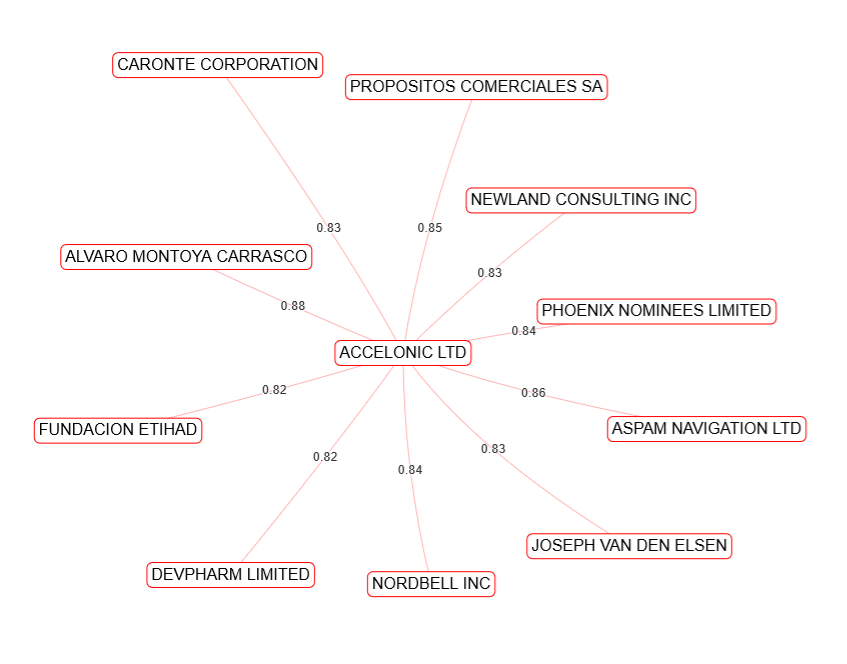
\includegraphics[width=9cm]{figures/accelonic_star.png}
    \caption{Direct similar nodes of the entity ACCELONIC LTD.}
    \label{fig:galaxy}
\end{figure}
Indeed, RDFsim can also create bigger networks, called similarity networks, for a given entity. In the corresponging figure, we have created the similarity graph for ACCELONIC LTD. We can use this graph to discover connections between nodes that are not necessarily connected in the original dataset.
\begin{figure}[htp]
    \centering
    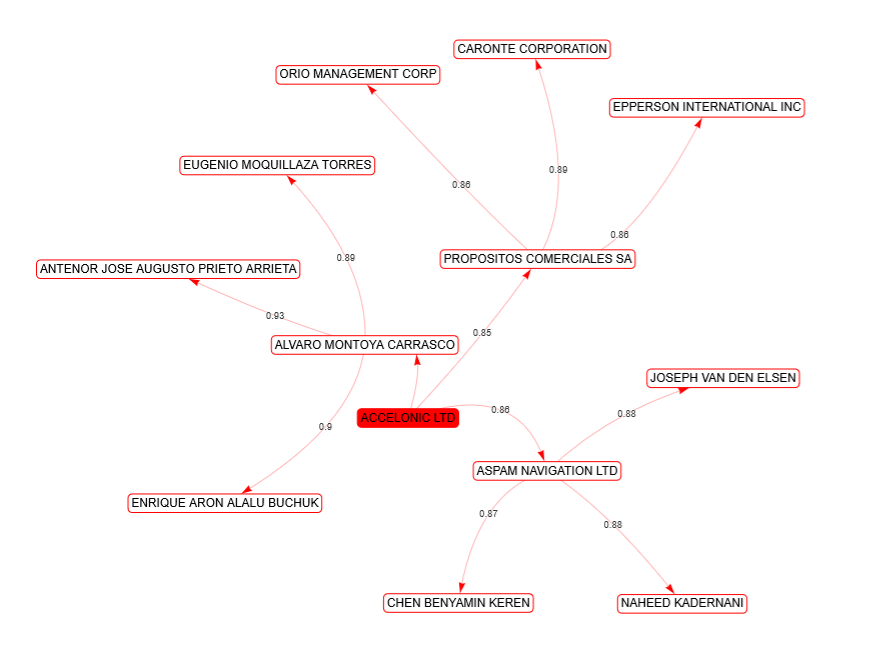
\includegraphics[width=8cm]{figures/accelonic_depth2.png}
    \caption{The similarity network of ACCELONIC LTD. The direction of the edges is the flow of similarity, while the labels of the edges are the cosine similarity between the nodes}
    \label{fig:galaxy}
\end{figure}
\\\textbf{[VELA GAS INVESTMENTS LTD.]} For this entity, we repeat the same steps as previously. 
\begin{figure}[htp]
    \centering
    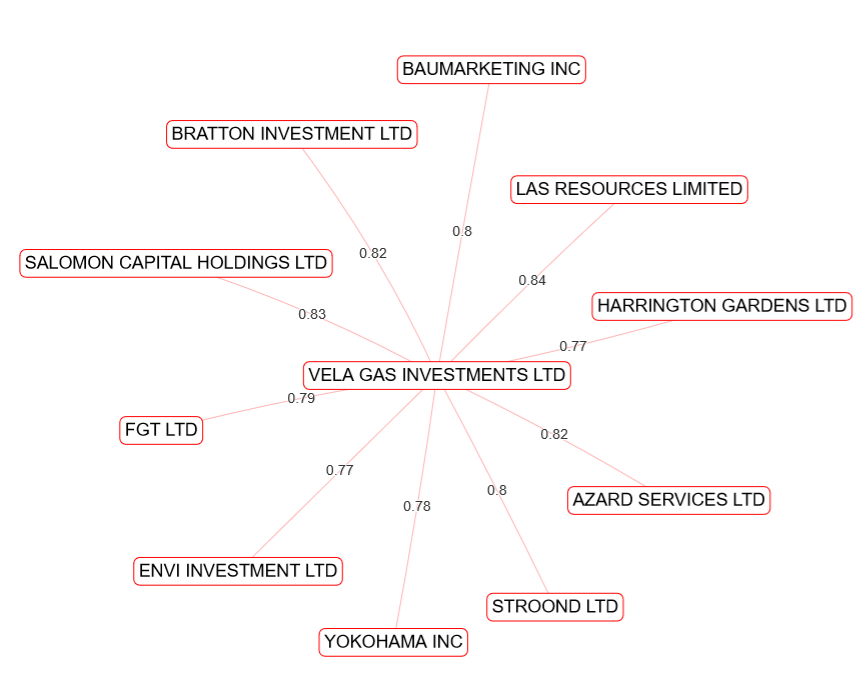
\includegraphics[width=8cm]{figures/vela_gas_star.png}
    \caption{Direct similar nodes of the entity VELA GAS INVESTMENTS LTD.}
    \label{fig:galaxy}
\end{figure}
\begin{figure}[htp]
    \centering
    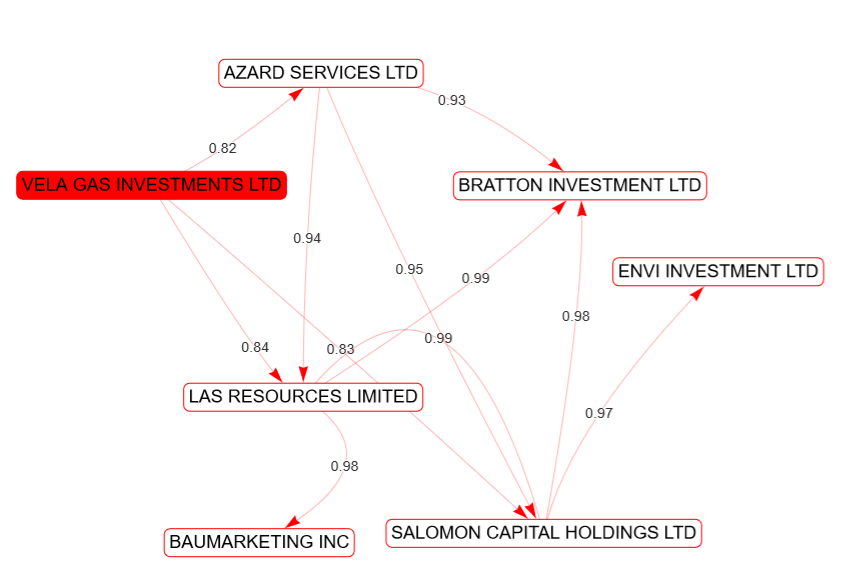
\includegraphics[width=8cm]{figures/vela_gas_depth2.png}
    \caption{The similarity network of VELA GAS INVESTMENTS LTD. The direction of the edges is the flow of similarity, while the labels of the edges are the cosine similarity between the nodes}
    \label{fig:galaxy}
\end{figure}
%\\\textbf{[ORION HOUSE SERVICES (HK) LIMITED]} For this entity, we repeat the same steps as previously. 
\\\textbf{[ORION HOUSE SERVICES (HK) LIMITED]} For this entity, we repeat the same steps as previously.
\begin{figure}[htp]
    \centering
    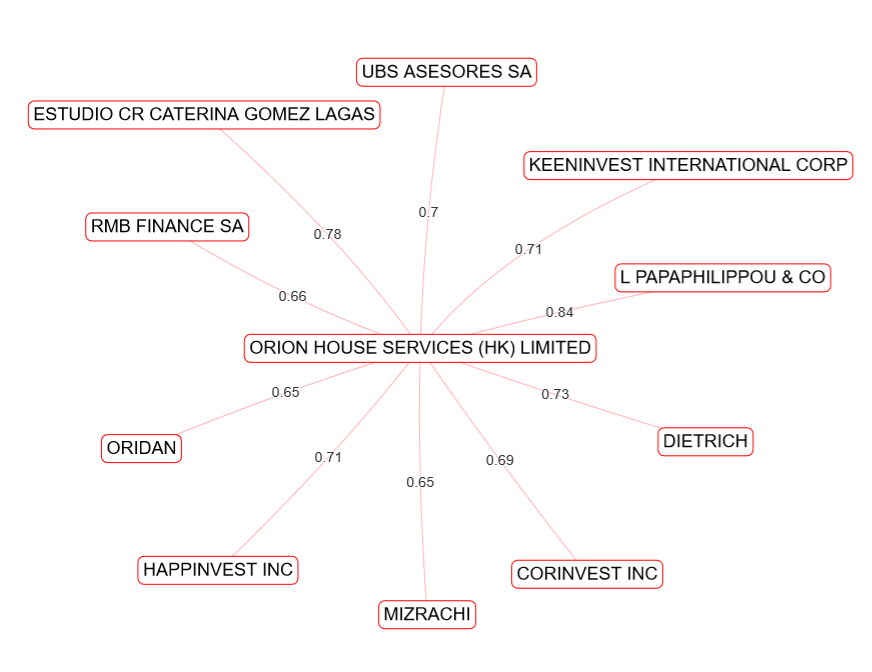
\includegraphics[width=8cm]{figures/orion_star.png}
    \caption{Direct similar nodes of the entity ORION HOUSE SERVICES (HK) LIMITED}
    \label{fig:galaxy}
\end{figure}
%We also create the similarity network.
\begin{figure}[htp]
    \centering
    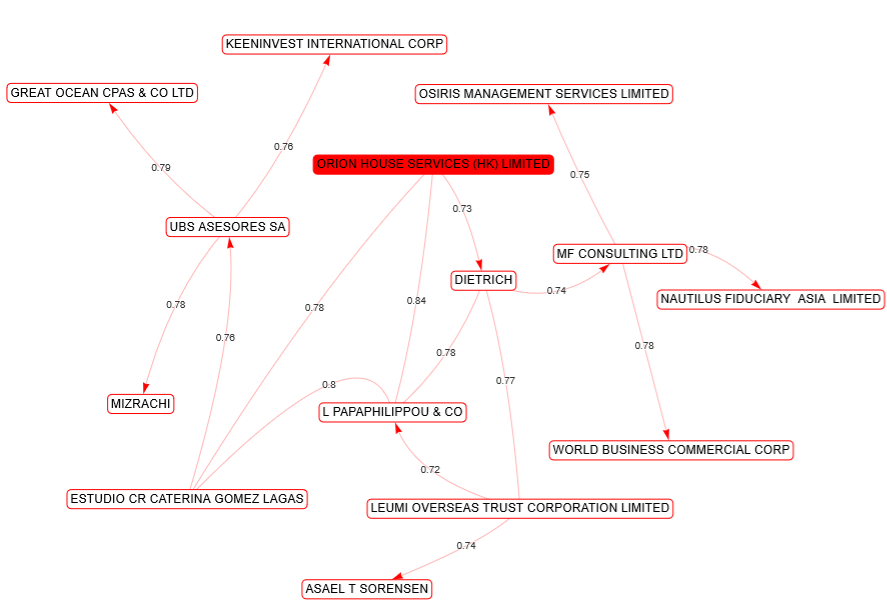
\includegraphics[width=8cm]{figures/orion_network_depth3.png}
    \caption{The similarity network of ORION HOUSE SERVICES (HK) LIMITED. The direction of the edges is the flow of similarity, while the labels of the edges are the cosine similarity between the nodes}
    \label{fig:galaxy}
\end{figure}

\subsubsection{Understanding the results}
Lets look at the similarity network of ACCELONIC LTD. Using this network, we can discover connections between offshores and other entities that were not clear before. For example, we see that our current node has high similarity score with ASPAM NAVIGATION LTD. This result could mean that these two nodes may have connections to similar entities, officers, companies and more. Given that our base data are dense and might have many connections between nodes, it could be difficult to discover such connections, or even worse, such connections might not even exist in the starting dataset. Exploiting graph embeddings for such graphs could actually offer a new way to discover relationships between the nodes of the graph, group offshores with same fraudulent activity and more, as shown in figure \ref{fig:useCase}.

\section{Conclusion}
This report presented multiple methods to analyze the data harvested from the fraud detection graph of the Panama papers leak. We tried to develop methods to efficiently study subsets of big datasets, while we managed to get results about important entities of the graph using graph analysis algorithms and visualizations. Last but not least, we proposed an alternative method to interact with the data and find patterns between nodes of the graph through embeddings and similarity search, while we proposed a port of our data in the RDFsim search engine. All the work done and resources used are available through the repository of the report \cite{panamaPapersAnalysis}.


\begin{figure}[htp]
    \centering
    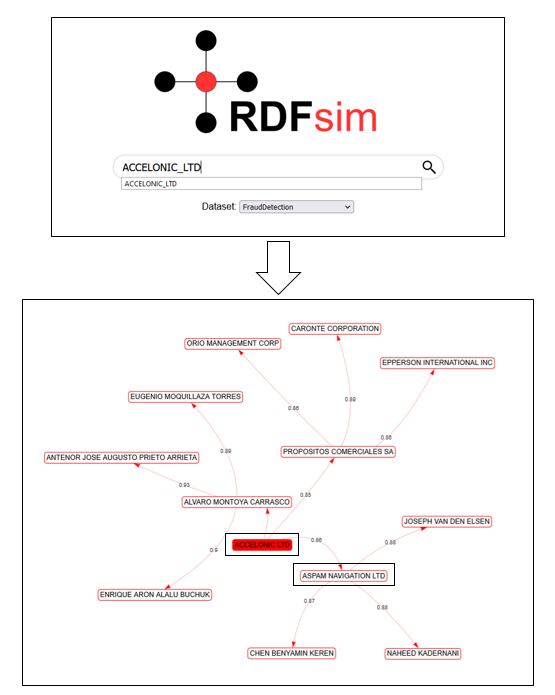
\includegraphics[width=6cm]{figures/useCase.png}
    \caption{Understanding the results for the similarity network of ACCELONIC LTD.}
    \label{fig:useCase}
\end{figure}

%\bibliographystyle{ACM-Reference-Format}
%\bibliography{sample}
\pagebreak
\printbibliography %Prints bibliography


\end{document}
\endinput
